\documentclass{article}
\usepackage{amsmath}
\usepackage{mathtools}
\usepackage{gensymb}
\usepackage[a4paper,inner=1.5cm,outer=1.5cm,top=2cm,bottom=0.5cm]{geometry} 
\usepackage{xcolor}
\usepackage{tikz}
\usepackage{multicol}
\usepackage{pgfplots}
\usetikzlibrary{intersections}
\usetikzlibrary{intersections,calc,angles,quotes}
\usetikzlibrary{calc,angles,positioning,intersections,quotes,decorations.markings}
\usepackage{tkz-euclide}
\usetikzlibrary{backgrounds}
\usetikzlibrary{calc,through}
\usetikzlibrary{angles}
\usetikzlibrary{fadings}
\usetikzlibrary{shapes.geometric}
\usetikzlibrary{shapes.symbols}
\usepackage{draftwatermark}
\usepackage{mathptmx}

\SetWatermarkText{\textcolor{black!10}{Mathema Shukur}}
\SetWatermarkFontSize{2 cm}
\usepackage[utf8]{inputenc}
\usepackage{fontspec}

\setmainfont{[Kalpurush.ttf]}
\newfontface{\en}{[Arial.ttf]} %%this is optional, if you want to use a secondary font. Any english font is supported
\newlength\Radius
\setlength\Radius{4cm}
\begin{document} 
	\Large
	\textcolor{red}{Welcome To} 
	\\
	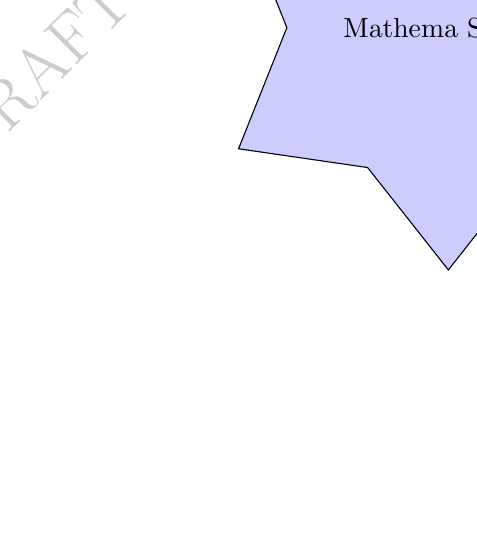
\begin{tikzpicture}
		\tikz \node [fill=blue!20,star,star points=6,draw] {Mathema Shukur };
	\end{tikzpicture}
	\\
	যাদের জন্যে প্রযোজ্যঃ  	\textcolor{magenta}{একাদশ ও দ্বাদশ শ্রেণীর শিক্ষার্থী} \\
	বিষয়ঃ \textcolor{magenta}{উচ্চতর গণিত ১ম পত্র} \\
	অধ্যায়ঃ \textcolor{magenta}{৩-সরলরেখা}\\ 
	Subtopicঃ  \textcolor{magenta}{ কার্তেসীয় সমীকরণ গঠন  করা }\\
	\\
	\\
	$\textcolor{blue}{x=r\,\,\cos \theta}$,\quad $\textcolor{blue}{y=r\,\,\sin \theta}$,\quad $\textcolor{blue}{r^2=x^2+y^2}$ \\
	\\
	\vspace{2cm}
	\\
	বাংলাদেশ টেক্সটাইল বিশ্ববিদ্যালয় ভর্তি পরীক্ষা- ২০১২-২০১৩\\
	(১)  $r=a\,\,\sin \theta$ এর কার্তেসীয় সমীকরণ নির্ণয় কর 
	\begin{align*}
		r&=a\,\,\sin \theta\\
		\\
		r^2&=a\,\,r\,\,\sin \theta\\
		\\
		x^2+y^2&=a \,\,y\\
		\\
		x^2+y^2-a\,\,y&=0
	\end{align*}
\\
\vspace{3cm}
\\
কুমিল্লা বোর্ড-২০০৮\\
(২)  $r(1+\cos \theta)=2$ এর কার্তেসীয় সমীকরণ নির্ণয় কর\\ 
\begin{align*}
	r(1+\cos \theta)&=2\\
	\\
	r+r\,\,\cos \theta&=2\\
	\\
	r+x&=2\\
	\\
	r&=2-x\\
	\\
	r^2&=(2-x)^2\\
	\\
	x^2+y^2&=4-4x+x^2\\
	\\
	y^2&=4-4x
\end{align*}
\\
ঢাকা বিশ্ববিদ্যালয় ভর্তি পরীক্ষা-২০১৮-২০১৯\\
(৩)  $2\,\,r\,\,\sin^2 \left(\frac{\theta}{2}\right)=1$ এর কার্তেসীয় সমীকরণ নির্ণয় কর \\ 
\begin{align*}
	2\,\,r\,\,\sin^2 \left(\frac{\theta}{2}\right)&=1\\
	\boxed{\textcolor{blue}{2\sin^2 A=1-\cos 2A}}&\\
	r\,\,(1-\cos \theta)&=1\\
	\\
	r-r\,\,\cos \theta &=1\\
	\\
	r-x&=1\\
	\\
	r&=1+x\\
	\\
	r^2&=(1+x)^2\\
	\\
	x^2+y^2&=1+2x+x^2\\
	\\
	y^2&=1+2x
\end{align*}
\\
শাহজালাল বিজ্ঞান ও প্রযুক্তি বিশ্ববিদ্যালয় ভর্তি পরীক্ষা-২০১৭-২০১৮\\ 
(৪)  $r\,\,\cos \left(\frac{\pi}{4}-\theta\right)=6$ এর কার্তেসীয় সমীকরণ নির্ণয় কর \\ 
\begin{align*}
	r\,\,\cos \left(\frac{\pi}{4}-\theta\right)&=6\\
	\boxed{\textcolor{blue}{\cos (A-B)=\cos A\,\,\cos B+\sin A\,\,\sin B}}&\\ 
	r\,\,\left[\cos \frac{\pi}{4}\,\,\cos \theta +\sin \frac{\pi}{4} \sin \theta\right]&=6\\
	\\
	r\,\,\left[ \frac{1}{\sqrt{2}}\,\,\cos \theta + \frac{1}{\sqrt{2}} \sin \theta\right]&=6\\
	\\
	 \frac{r\,\,\cos \theta}{\sqrt{2}} + \frac{r\,\,\sin \theta}{\sqrt{2}} &=6\\
	 \\
	 \frac{x}{\sqrt{2}} + \frac{y}{\sqrt{2}} &=6\\
	 \\
	 x+y&=6\sqrt{2}
\end{align*}
\end{document}